\chapter{Implementation}\label{ch:implementation}

\section{Output Switch Matrix}\label{sec:osm}
\subsection{Description}
The different boards must route the data differently to the FEX systems depending on the detector region they are connected to. To tackle this problem, either each LATOME has a different version of the firmware, or some code must be added to allow an online configuration procedure defining the routing. The second possibility was chosen in the LAr group, and the solution proposed by Marcos for the V6 firmware was to add an Output Switch Matrix. 

The OSM uses multiplexers to route the 17 inputs to the 48 outputs and takes its selection bits from registers configured online via an ipbus. The HLS implementation is very simple, mainly involving a 2D array with 48 rows made of a subgroup of the 17 possible inputs.

\begin{figure}
    \centering
    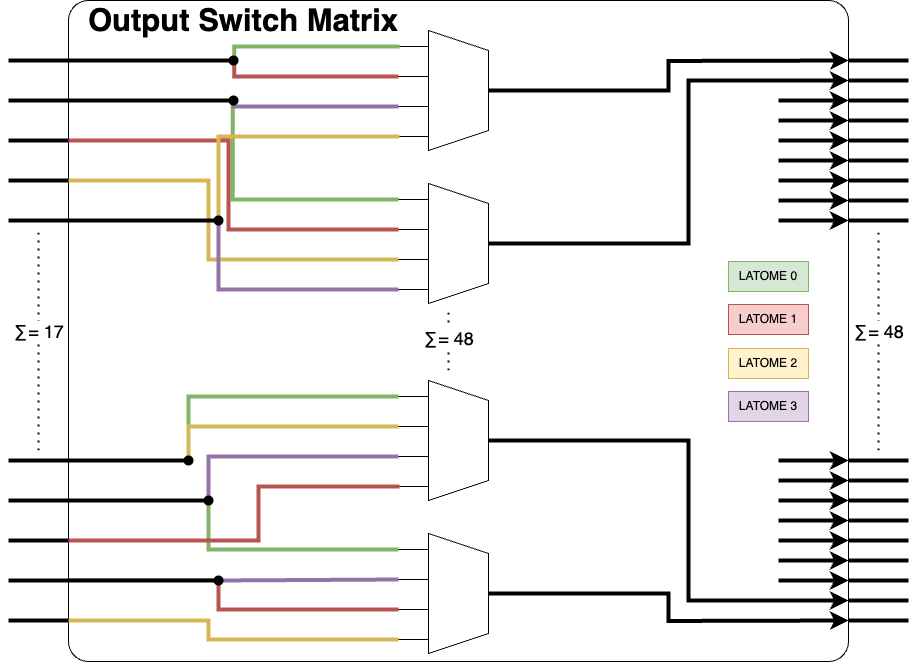
\includegraphics[width=1\textwidth]{osm.png}
    \caption{Output Switch Matrix Simplified Diagram}
    \label{fig:original-vhdl-design}
\end{figure}

Without looking at the different LATOME routings, it appears that, there should be 48 multiplexers of input size \(224\times17=3808\).
However when considering the data paths and optimizing for them, the biggest multiplexers have at most 4 input frames, meaning that each row from the HLS 2D array have 4 entries.
Figure \ref{fig:osum-v6} shows the parallel to serial block creating 32 bits words for the FEX systems. Moving this block to the left would have no impact on the latency. However, by moving this block before the Output Switch Matrix, the biggest multiplexers would have an input size of \(4\times32\) instead of \(4\times224\).

An important aspect to monitor is the data dependencies, since these could have a critical impact if using TDM. The OSM block is a routing block which does not change any data in the frames. The Frame Alignment only overwrites the data that it gets as input if the current BC index is an alignment one, hence it does not show data dependencies. Finally the Cyclic Redundant Check can be both computed in a parallel or serial fashion equivalently and only depends on the CRC temporary result from time \(t=-1\).

\subsection{Serializing Before the OSM}

Serializing the 224-bit full frames to 32-bit words requires 7 clock cycles, as \(224/7=32\). Hence the operating frequency of the OSUM block must be \(7\times40=280MHz\).


\section{Optimizing the HLS Directives}
